\documentclass{oci}
\usepackage[utf8]{inputenc}
\usepackage{lipsum}
\usepackage{tikz}
\usetikzlibrary{calc}

\title{Escaleras y Serpientes}

\begin{document}
\begin{problemDescription}
  Escaleras y Serpientes es un popular juego de mesa que por décadas ha
  llenado de diversión las tardes de grandes y pequeños.
  El juego original consta de un tablero de $10\times 10$ casillas numeradas de
  1 a 100 como se muestra en la imagen de más abajo.
  Los jugadores parten con una ficha en la primera casilla y se turnan para
  lanzar un dado que les indicará la cantidad de casillas que deben avanzar.
  Las fichas se mueven según la numeración del tablero, en sentido ascendente.
  Si al finalizar un movimiento un jugador cae en una casilla donde comienza una
  escalera, sube por ella hasta la casilla donde esta termina.
  Si, por el contrario, cae en una en donde comienza la cabeza de una serpiente,
  desciende por esta hasta la casilla donde finaliza su cola.
  El primero en llegar a la última casilla, marcada con una estrella en la
  imagen de abajo, es quién gana el juego.

  \begin{center}
  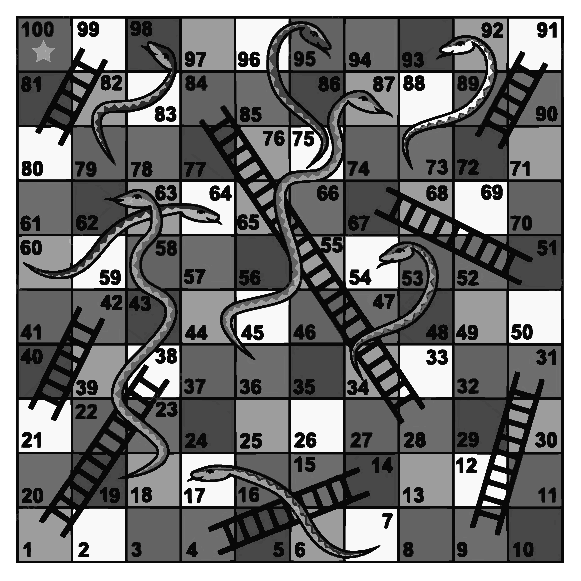
\includegraphics[scale=0.8]{tablero}
  \end{center}

  Por motivo del aniversario del juego, algunos desarrolladores está intentando
  lanzar una versión para computador.
  En esta versión, los jugadores pueden escoger la cantidad de filas, $M$, y de
  columnas, $N$, en el tablero.
  Las filas en el tablero se enumeran de abajo hacia arriba entre 0 y $M-1$, y
  las columnas de izquierda a derecha entre 0 y $N-1$.
  Cada casilla del tablero puede identificarse con un par $(a, b)$ donde $a$
  corresponde a su fila y $b$ a su columna.
  La figura que se ve a continuación muestra la forma de identificar cada
  casilla en un tablero de 4 filas por 5 columnas.
  Las casillas se recorren de la misma forma que en el juego original avanzando
  hacia la derecha en las filas pares y hacia la izquierda en las impares.

  \begin{center}
    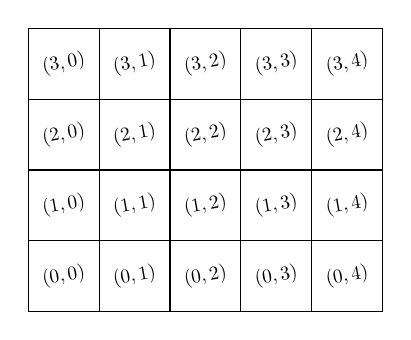
\begin{tikzpicture}[scale = 0.6]
      \foreach \i in {0,...,4}{
        \foreach \j in {0,...,3}{
          \draw (1.5*\i,1.5*\j) rectangle +(1.5,1.5);
          \node at (1.5*\i + 0.75,1.5*\j + 0.75) [rotate=10] {\scalebox{0.7}{$(\j, \i)$}};
        }
      }
    \end{tikzpicture}
    ~
    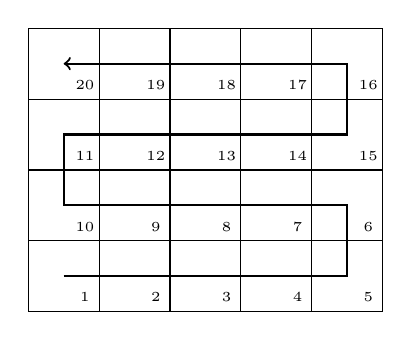
\begin{tikzpicture}[scale = 0.6]
      \foreach \i in {0,...,4}{
        \foreach \j in {0,...,3}{
          \draw (1.5*\i,1.5*\j) rectangle +(1.5,1.5);
          \node at (1.5*\i + 1.2,1.5*\j + 0.3) {
            \tiny
            \pgfmathparse{Mod(\j,2)==0?1:0}
            \ifnum\pgfmathresult>0
                \pgfmathtruncatemacro\result{\j*5+\i+1}\result
            \else
                \pgfmathtruncatemacro\result{\j*5-\i+5}\result
            \fi
          };
        }
      }
      \draw [->, thick]
              (0.75, 0.75) -- (6.75, 0.75) --
              (6.75, 2.25) -- (0.75, 2.25) --
              (0.75, 3.75) -- (6.75, 3.75) --
              (6.75, 5.25) -- (0.75, 5.25);
    \end{tikzpicture}
  \end{center}

  Los desarrolladores llevan gran parte del juego programado pero están teniendo
  problemas con el módulo que mantiene actualizada la posición de cada ficha.
  Dada la descripción de un tablero y el resultado que un jugador obtiene en un
  dado en cada turno tu tarea es determinar en que casilla termina este jugador.
\end{problemDescription}

\begin{inputDescription}
  La entrada comienza con una línea conteniendo dos enteros $M$ y $N$ ($2 \leq
  M, N \leq 1000$), correspondientes respectivamente a la cantidad de filas y
  columnas en el tablero.
  La siguiente línea contiene un entero $E$ ($E \geq 0$) correspondiente a la
  cantidad de escaleras y serpientes.
  Cada una de las siguientes $E$ líneas describe uno de los objetos en el
  tablero (escaleras o serpientes).
  Cada objeto está descrito con cuatro enteros $a, b, c$ y $d$ ($0 \leq a, c
  \leq M, 0 \leq b, d \leq N$)
  representando que el objeto comienza en la casilla $(a, b)$ y termina en la
  casilla $(c, d)$.
  No habrán nunca dos objetos que comiencen en la misma casilla y un objeto
  nunca comenzará en la casilla que termina otro.

  A continuación viene una línea con un entero $T$ ($T > 0$) conteniendo la
  cantidad de turnos.
  Finalmente, la última línea contiene $T$ enteros mayores o iguales que 1 y
  menores o iguales 6, correspondientes al resultado del dado en cada turno.
\end{inputDescription}

\begin{outputDescription}
  La salida debe contener una línea con dos enteros correspondientes a la
  columna y fila, de la posición donde termina el jugador.
\end{outputDescription}

\begin{scoreDescription}
  \score{10} Se probarán varios casos donde el tablero no contiene ninguna
  escalera ni serpiente y la cantidad de turnos es menor o igual que 100
  ($E = 0$, $T \leq 100$).
  \score{10} Se probarán varios casos donde la cantidad de escaleras y
  serpientes es menor o igual que 100 y la cantidad de turnos es menor o igual
  que $10^4$ ($E \leq 100$, $T \leq 10^4$)
  \score{10} Se probarán varios caso donde la cantidad de escaleras y serpientes
  es menor o igual que 5000 y la cantidad de turnos es menor o igual que $10^5$
  ($E \leq 5000$, $T \leq 10^5$)
\end{scoreDescription}

\begin{sampleDescription}
\sampleIO{sample-1}
\sampleIO{sample-2}
\end{sampleDescription}

\end{document}
